\chapter[Parte II --- Sistema de rastreo]{Parte II --- Sistema de rastreo de ubicaci\'on por consentimiento}
\label{ch:parte2}
\tagbox{tagrealc}{CÓDIGO Y PRUEBAS REALES}

\section{Enfoque}

Ninguna técnica legítima permite ubicar un teléfono a partir de su número sin la cooperación del titular o de la operadora. WhatsApp y Telegram no exponen la ubicación de sus usuarios a terceros; solo la comparten cuando el propio usuario la envía. El sistema se diseñó en consecuencia: \textbf{solo registra la ubicación que el titular del número envía voluntariamente}, después de aceptar el consentimiento y verificar el número con un código de un solo uso, y le permite pausar el rastreo o borrar sus datos en cualquier momento.

Casos de uso previstos: compartir ubicación entre familiares, seguimiento de flotas con conocimiento del conductor, acompañamiento de trayectos.

\section{Arquitectura}

\begin{figure}[htbp]
  \centering
  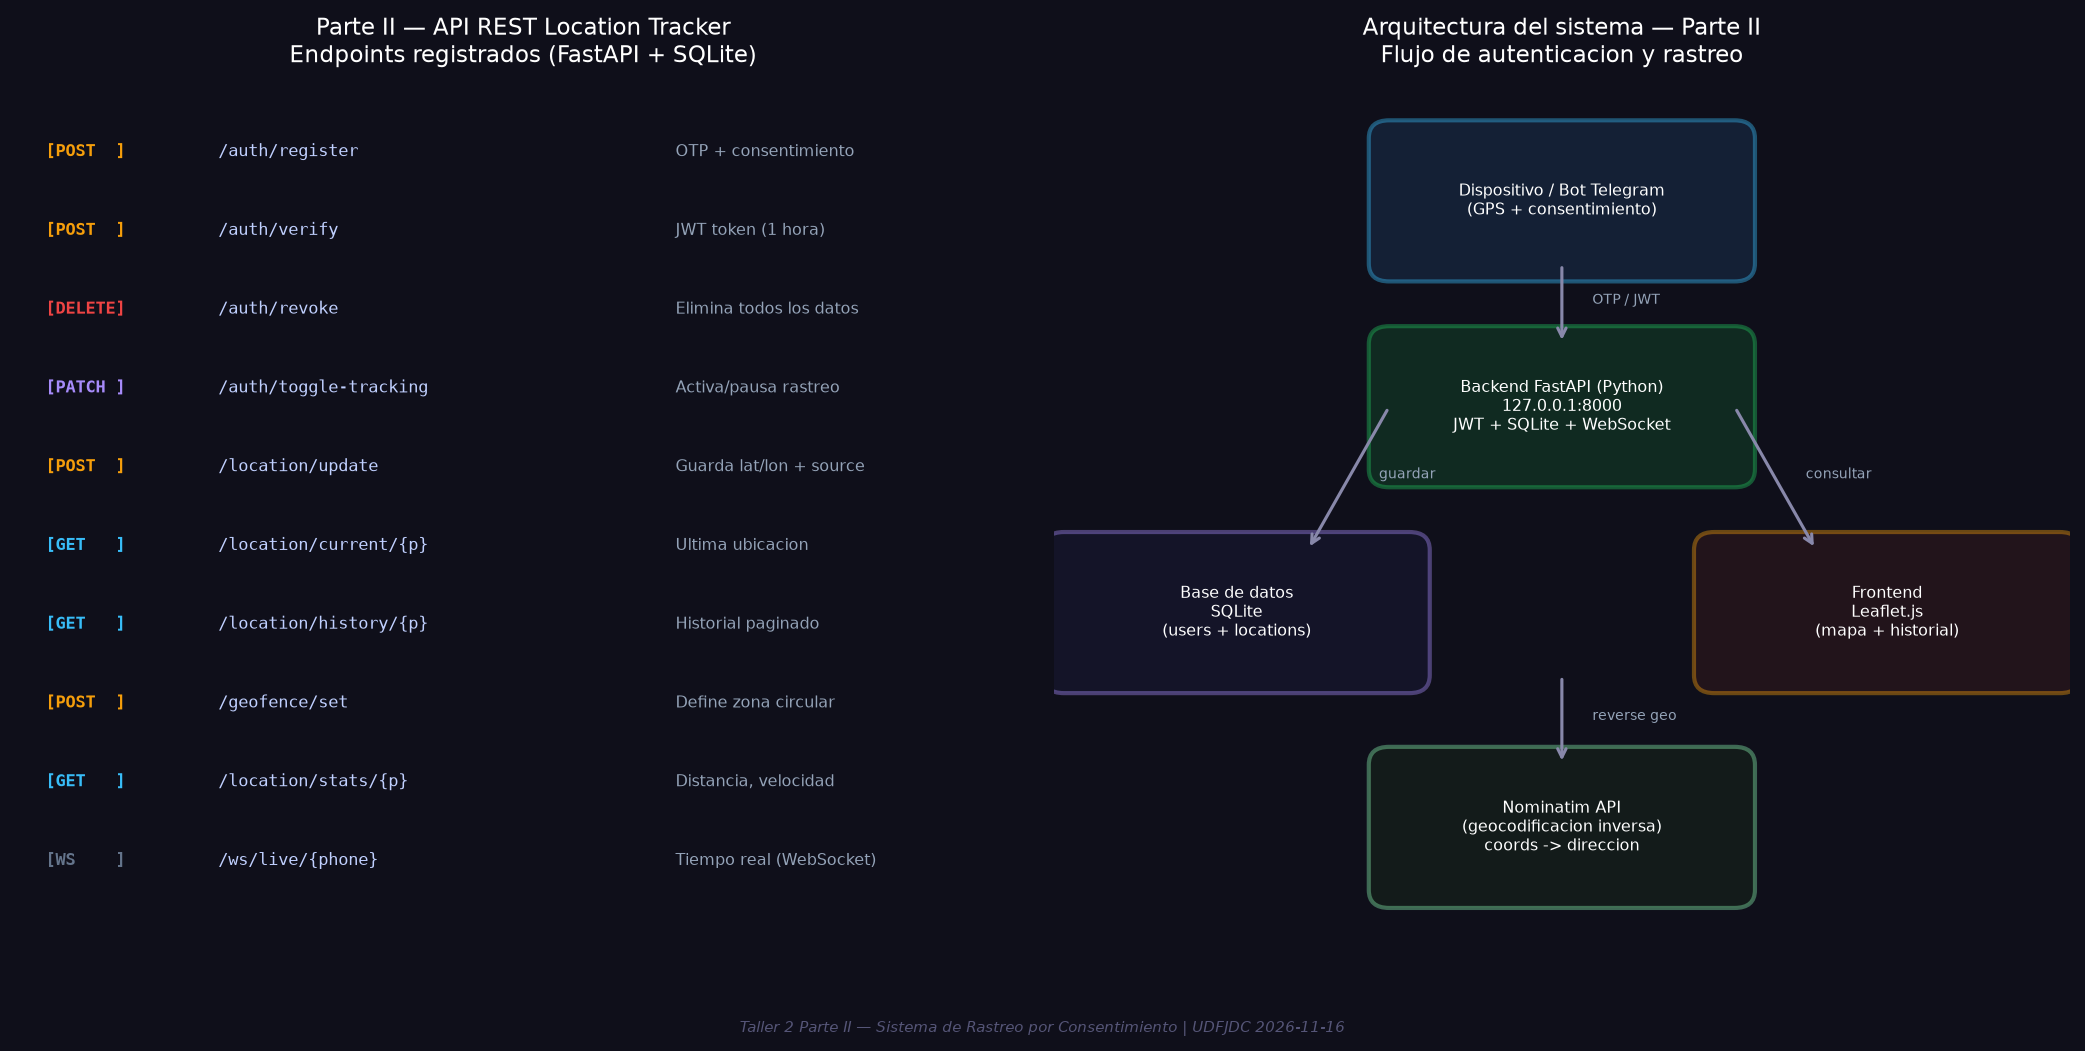
\includegraphics[width=0.92\linewidth,height=0.82\textheight,keepaspectratio]{figures/parte2_sistema_funcionando.png}
  \caption[Endpoints de la API y arquitectura: dispositivo o bot de Telegram,\ldots{}]{Endpoints de la API y arquitectura: dispositivo o bot de Telegram, backend FastAPI, base de datos SQLite, panel web con Leaflet y geocodificación inversa.}
\end{figure}

\begin{table}[H]
\centering
\small
\caption[Arquitectura (tabla 1)]{Arquitectura}
\begin{tabularx}{\linewidth}{>{\raggedright\arraybackslash}X >{\raggedright\arraybackslash}X >{\raggedright\arraybackslash}X >{\raggedright\arraybackslash}X}
\toprule
\textbf{Componente} & \textbf{Archivo} & \textbf{Tecnología} & \textbf{Función} \\
\midrule
Backend & \texttt{\seqsplit{parte2/\allowbreak{}backend/\allowbreak{}main.py}} & FastAPI, JWT (HS256), WebSocket & Registro, verificación, recepción y consulta de ubicaciones \\
Datos & \texttt{\seqsplit{parte2/\allowbreak{}backend/\allowbreak{}database.py}} & SQLAlchemy sobre SQLite & Tablas \texttt{users} y \texttt{location\_records} \\
Panel web & \texttt{\seqsplit{parte2/\allowbreak{}frontend/\allowbreak{}index.html}} & Leaflet y OpenStreetMap & Mapa, última ubicación, historial y trazado de ruta \\
Bot & \texttt{\seqsplit{parte2/\allowbreak{}telegram\_bot/\allowbreak{}bot.py}} & python-telegram-bot & Consentimiento, verificación y envío de ubicación desde Telegram \\
\bottomrule
\end{tabularx}
\end{table}

\section{Flujo de uso}

\begin{enumerate}
  \item El usuario acepta el consentimiento y registra su número (\texttt{POST /auth/register}). El backend guarda la fecha de aceptación y genera un OTP de seis dígitos con vigencia de 10 minutos.
  \item Verifica el OTP (\texttt{POST /auth/verify}) y recibe un token JWT válido por 60 minutos.
  \item Envía su ubicación (\texttt{POST /location/update}) desde el bot, con el botón \guillemotleft{}Compartir mi ubicación\guillemotright{}, o desde cualquier cliente con el token.
  \item El panel consulta la última posición y el historial, dibuja el recorrido y recibe actualizaciones por WebSocket.
  \item El usuario puede pausar el rastreo (\texttt{PATCH /auth/toggle-tracking}) o revocar el consentimiento y borrar todo (\texttt{DELETE /auth/revoke}).
\end{enumerate}

\section{Evidencia de funcionamiento}

\textbf{Prueba de la API} ejecutada en el equipo local (127.0.0.1:8000) el 2026-11-16 a las 21:50 (UTC-5), con el número de demostración +57 300 123 4567:

\begin{table}[H]
\centering
\small
\caption[Evidencia de funcionamiento (tabla 1)]{Evidencia de funcionamiento}
\begin{tabularx}{\linewidth}{>{\raggedright\arraybackslash}X >{\raggedright\arraybackslash}X >{\raggedright\arraybackslash}X}
\toprule
\textbf{\#} & \textbf{Petición} & \textbf{Resultado} \\
\midrule
1 & \texttt{POST /\allowbreak{}auth/\allowbreak{}register} & OTP generado: 679470 \\
2 & \texttt{POST /\allowbreak{}auth/\allowbreak{}verify} & Token JWT emitido \\
3 & \texttt{POST /\allowbreak{}location/\allowbreak{}update} (2 veces) & Registros 1 y 2 creados \\
4 & \texttt{\seqsplit{GET /\allowbreak{}location/\allowbreak{}current/\allowbreak{}\{phone\}}} & lat 4,615, lon $-$74,075 \\
5 & \texttt{\seqsplit{GET /\allowbreak{}location/\allowbreak{}stats/\allowbreak{}\{phone\}}} & 2 registros, 0,948 km \\
6 & \texttt{\seqsplit{GET /\allowbreak{}location/\allowbreak{}history/\allowbreak{}\{phone\}}} & 2 registros \\
7 & \texttt{POST /\allowbreak{}geofence/\allowbreak{}set} & Zona 4,6097, $-$74,0817, radio 500 m \\
8 & \texttt{\seqsplit{PATCH /\allowbreak{}auth/\allowbreak{}toggle-tracking?enabled=false}} & Rastreo pausado \\
\bottomrule
\end{tabularx}
\end{table}

La base de datos que dejó esa prueba confirma cada paso: un usuario verificado, con fecha de consentimiento, OTP ya consumido, rastreo pausado, zona definida y dos ubicaciones almacenadas (las horas de la base están en UTC).

\begin{figure}[htbp]
  \centering
  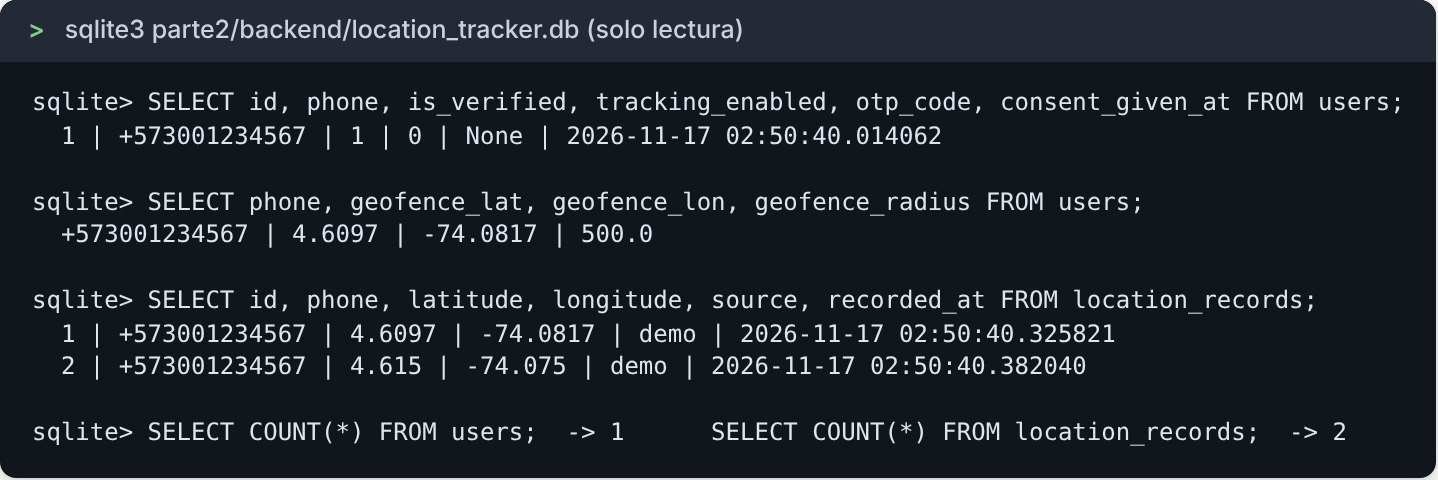
\includegraphics[width=\linewidth,height=0.82\textheight,keepaspectratio]{figures/cap_parte2_base_datos.png}
  \caption[Consulta de solo lectura a \texttt{location\_tracker.db} tras la prueba:\ldots{}]{Consulta de solo lectura a \texttt{location\_tracker.db} tras la prueba: usuario verificado con consentimiento, zona de geofencing y dos registros de ubicación.}
\end{figure}

\begin{figure}[htbp]
  \centering
  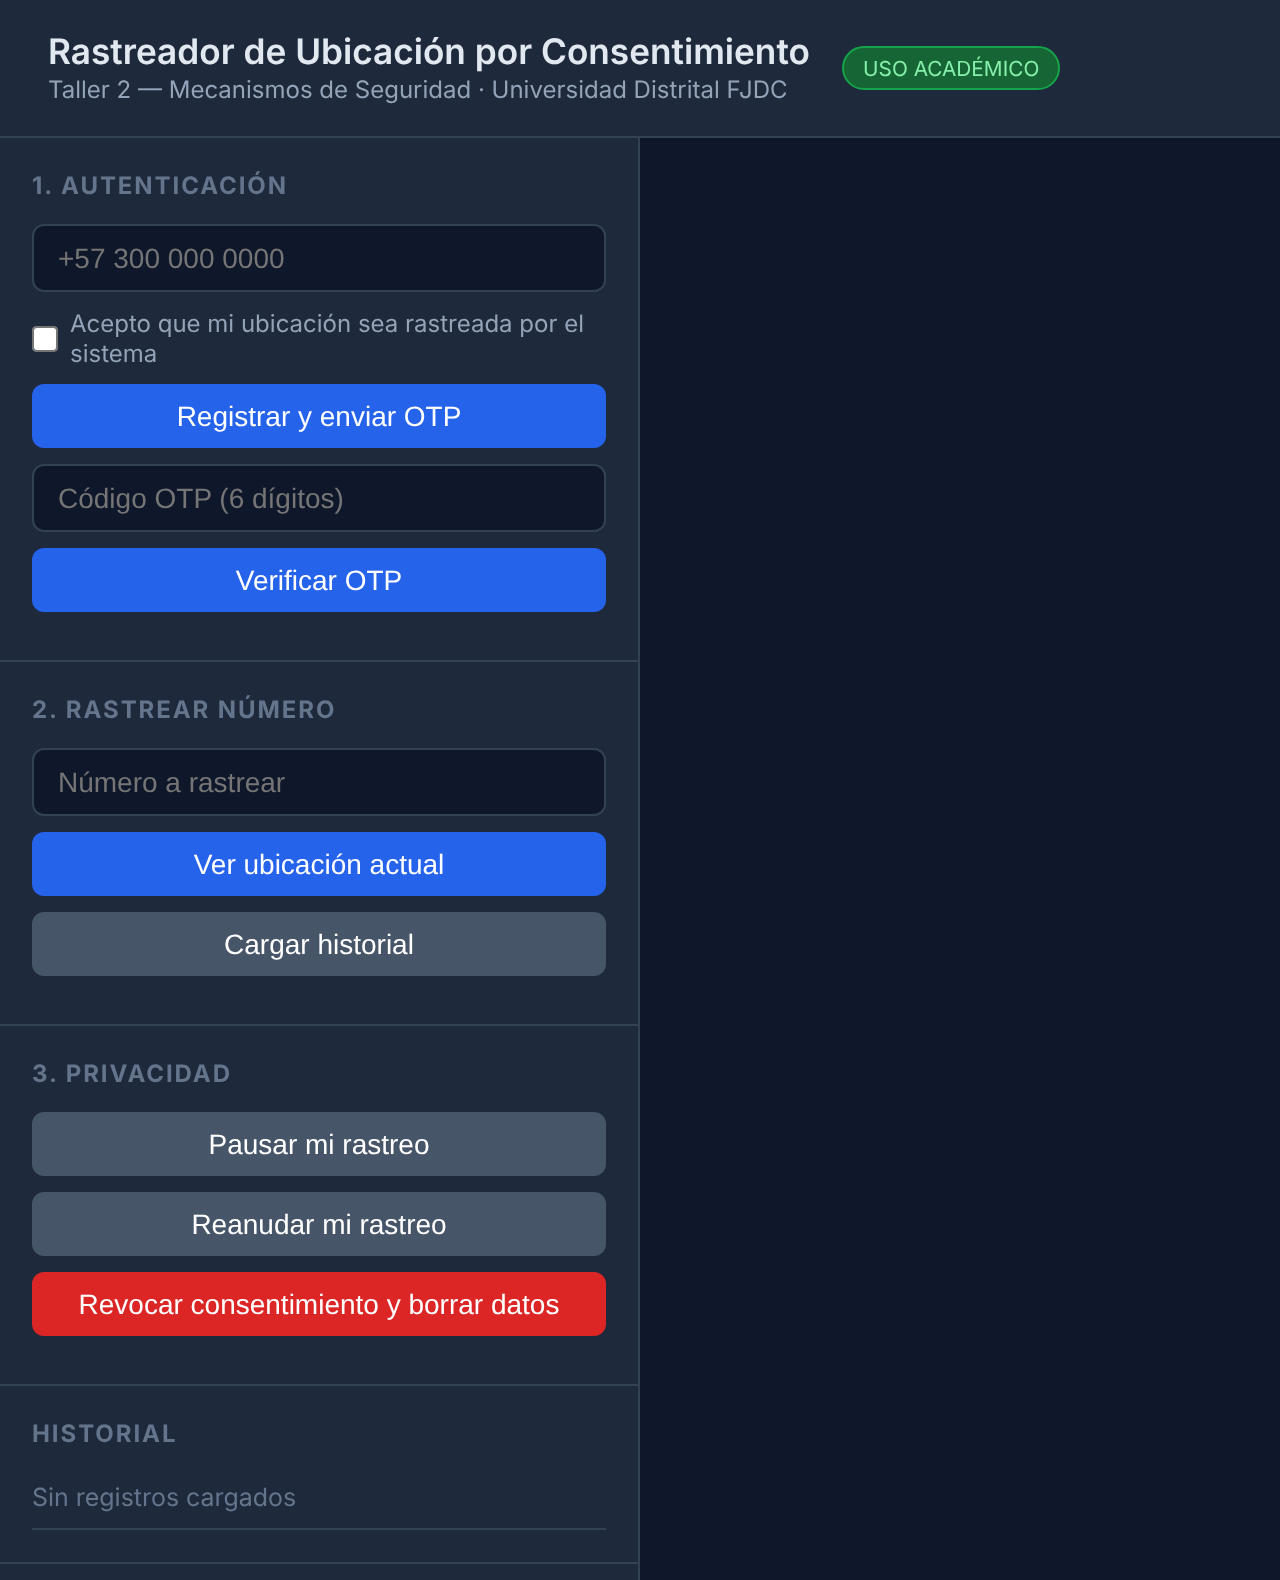
\includegraphics[width=0.52\linewidth,height=0.82\textheight,keepaspectratio]{figures/cap_parte2_frontend_panel.png}
  \caption[Panel web real (\texttt{frontend/index.html}) abierto en Chrome:\ldots{}]{Panel web real (\texttt{frontend/index.html}) abierto en Chrome: autenticación con casilla de consentimiento, consulta de ubicación, controles de privacidad e historial. El área del mapa se omite porque necesita conexión a Internet para cargar Leaflet y las teselas de OpenStreetMap.}
\end{figure}

\section{Cobertura de requisitos}

\begin{table}[H]
\centering
\small
\caption[Cobertura de requisitos (tabla 1)]{Cobertura de requisitos}
\begin{tabularx}{\linewidth}{>{\raggedright\arraybackslash}X >{\raggedright\arraybackslash}X >{\raggedright\arraybackslash}X}
\toprule
\textbf{Requisito de la guía} & \textbf{Estado} & \textbf{Cómo se cumple o qué falta} \\
\midrule
Registro por número telefónico & Cumplido (demo) & Registro con OTP. El código se devuelve en la respuesta en lugar de enviarse por SMS \\
Solicitud y captura de ubicación & Cumplido & El usuario la envía desde el bot de Telegram o por la API \\
Actualización periódica & Parcial & La API acepta envíos sucesivos y el panel se actualiza por WebSocket; falta el cliente móvil que envíe cada N minutos \\
Visualización en mapa & Cumplido & Leaflet con OpenStreetMap; marcador y polilínea del recorrido \\
Geocodificación inversa & Cumplido & Consulta a Nominatim desde el panel \\
Alertas por zona (opcional) & Parcial & La zona se guarda con \texttt{/\allowbreak{}geofence/\allowbreak{}set}; falta evaluar entrada y salida y notificar \\
Historial de ubicaciones & Cumplido & Paginado con \texttt{limit} y \texttt{offset}; falta filtro por fecha \\
Acceso seguro & Parcial & OTP y JWT; ver hallazgos de seguridad \\
Bot de Telegram & Cumplido & Solicita contacto y ubicación con botones; no rastrea sin acción del usuario \\
Estadísticas de recorrido (opcional) & Cumplido & Distancia (Haversine), duración y velocidad media \\
Aplicación móvil Android/\allowbreak{}iOS & No implementado & El bot de Telegram cumple el papel de cliente en el dispositivo \\
\bottomrule
\end{tabularx}
\end{table}

\section{Revisión de seguridad del prototipo}

Aplicando al propio sistema los criterios de la Parte I, la revisión del código encontró estos puntos. Se documentan como trabajo pendiente antes de cualquier uso fuera del laboratorio.

\begin{table}[H]
\centering
\small
\caption[Revisión de seguridad del prototipo (tabla 1)]{Revisión de seguridad del prototipo}
\begin{tabularx}{\linewidth}{>{\raggedright\arraybackslash}X >{\raggedright\arraybackslash}X >{\raggedright\arraybackslash}X >{\raggedright\arraybackslash}X}
\toprule
\textbf{\#} & \textbf{Hallazgo} & \textbf{Riesgo} & \textbf{Corrección propuesta} \\
\midrule
1 & \texttt{\seqsplit{GET /\allowbreak{}location/\allowbreak{}current}}, \texttt{/\allowbreak{}history} y \texttt{/\allowbreak{}stats} aceptan cualquier número: basta un token válido propio para consultar la ubicación de otro usuario & \textbf{Alto.} Rompe el modelo de consentimiento & Autorizar solo al titular o a quienes él haya aprobado de forma explícita (tabla de permisos por observador) \\
2 & El WebSocket \texttt{/\allowbreak{}ws/\allowbreak{}live/\allowbreak{}\{phone\}} no pide autenticación & \textbf{Alto.} Cualquiera puede suscribirse a las actualizaciones de un número & Exigir el token al conectar y aplicar la misma autorización \\
3 & El OTP se devuelve en la respuesta y se guarda en claro; se genera con \texttt{random} & Medio. Aceptable solo en demostración & Enviar por SMS, guardar solo el hash, generar con \texttt{secrets} y limitar intentos \\
4 & \texttt{SECRET\_KEY} con valor por defecto en el código & Medio. Permite falsificar tokens si no se configura & Exigir la variable de entorno y fallar al arrancar si falta \\
5 & CORS con \texttt{\seqsplit{allow\_origins=["*"]}} y credenciales & Medio & Lista de orígenes permitidos \\
6 & Sin límite de tasa en registro y verificación & Medio. Fuerza bruta de un OTP de seis dígitos & Límite por número y por IP; bloqueo temporal \\
7 & El panel envía las coordenadas a Nominatim y carga teselas de OpenStreetMap & Bajo. Terceros reciben coordenadas & Informarlo en el consentimiento o usar un geocodificador propio \\
8 & Sin TLS en el entorno local & Bajo en laboratorio & Proxy inverso con HTTPS en cualquier despliegue \\
\bottomrule
\end{tabularx}
\end{table}

\section{Privacidad y marco legal}

\begin{itemize}
  \item El consentimiento queda registrado con fecha y hora y es requisito para crear la cuenta.
  \item El titular puede pausar el rastreo y ejercer la supresión completa de sus datos.
  \item En Colombia, la ubicación de una persona es un dato personal protegido por la Ley 1581 de 2012: su tratamiento exige autorización previa, expresa e informada, finalidad definida y la posibilidad de revocarla. Rastrear a alguien sin su conocimiento queda fuera del alcance de este sistema y de la guía.
  \item Mientras el hallazgo 1 no se corrija, el prototipo debe usarse únicamente con números de prueba.
\end{itemize}